 \documentclass[30pt,a4paper]{article}
% Dokumenten Typ, titelseite, Schriftgröße, Seitenformat
\PassOptionsToPackage{dvipsnames}{xcolor}
% Füge neue Farben hinzu (standart 5 farben oder so)
\usepackage[utf8]{inputenc}
% Kodierung
\usepackage[T1]{fontenc}
% Umlaute
\usepackage[german]{babel}
% Eingebundene Sprachen
\usepackage{graphicx}
% Einbinden von Grafiken
\usepackage{wrapfig}
% Text um kleine Grafiken herumsetzen
\usepackage{amsmath}
\usepackage{amsfonts}
\usepackage{amssymb}
% Mathe Symbole und Commands
\usepackage{mathtools}
% Verbessert ams Packete von oben
\usepackage{nicefrac}
% Schönere Brüche
\usepackage{tikz}
\usepackage{circuitikz}
\usepackage{tikz-cd}
% Tikz Stuff
\usepackage{enumerate}
% Bessere Aufzählungen
\usepackage{cancel}
% z.B Durchstreichen von Sachen
\usepackage[hidelinks]{hyperref}
\usepackage{cleveref}
% Links und Referenzen innerhalb des Dokuments
\usepackage{tcolorbox}
% Wunderschöne Farbige Boxen mit Überschriften
\usepackage{caption}
% Erstellen von captions innerhalb einer Minipage
\usepackage[margin=1in]{geometry}
% Änderung der Gestaltung einer Seite (Überschreibt \documentclass)
\usepackage{placeins}
% Mit Hilfe von \FloatBarrier floats einschränken
\usepackage{booktabs}
% Bei Tabellen wird kann anstelle von \hline \toprule, \midrule und \bottomrule verwendet werden etc.
\usepackage{wasysym}
% Fügt eine Reihe von Symbolen wie Männlich Weiblich dazu
\usepackage{url}
% Füge Problemlos urls ein



\hbadness=99999 
% Löst ein Problem mit \hbox

\newenvironment{Dtabular}[2][1] {\def\arraystretch{#1}\tabular{#2}}
{\endtabular}

\title{
	\large Fortgeschrittenes Physik Lab	SS19 \\[4mm]
	\textbf{\LARGE Experiment: Rastertunnel
	} \\[4mm]
	(Durchgeführt am: 18-19.09.19 bei Meinhardt Patrick) \\}
% Titel des Experiments
\author{Erik Bode, Damian Lanzenstiel \\ (Group 103)}
\date{28.September 2019}
% Autoren

\begin{document}
	
	\begin{titlepage}
		\maketitle
		\vspace{2cm}
		\begin{abstract}
			Im Versuch zum Rastertunnelmikroskop sollte die Oberfläche von unterschiedlichen Materialien untersucht werden. Hierzu wurden Graphit, Gold und Molybdändisulfid benutzt. Für Graphit sollte dann die Gitterkonstante bestimmt werden. Hierbei wurden ein Wert von $a=(0.2585\pm0.0019)\,\text{nm}$ für die Gitterkonstante herhalten. Jedoch ist dieser vermutlich wegen Systematischen Fehlern nicht mit dem Literaturwert von $a=0.2456\,$nm verträglich. Für Gold wurde eine wolkenartige Struktur gesehen die mit den Erwartungen übereinstimmt. Für Molybdändisulfid konnte keine passende Auflösung gefunden werden. 
		\end{abstract}
	\end{titlepage}
	\newpage
	\tableofcontents
	\newpage
	\section{Theory}
The contents of this chapter are, if not otherwise specified, derived from the guide to the experiment \cite{anleitung}
\subsection{Spin and nuclear spin}
The spin or intrinsic angular momentum of a elementary particle is an intrinsic property of particles from the family of the fermions. Members of this family, such as protons, neutrons and electrons all have a spin of $s=\frac{1}{2}$.
The spin can be explained semi classically, as rotation of the particle around its own 'centre of mass', with fixed frequency and variable axis of rotation. 
However, this illustration only makes sense in finite-size particles, of course. Just as with the angular momentum, not all three spin components can be defined at the same time, but only the amount and projection on a freely selectable 'quantization axis'.
The possible spin quantum numbers are $$ \left|\vec{S}\right| = \hbar \sqrt{S\left(S+1\right)}$$ with $S = 0, \frac{1}{2}, 1, ...$ and Planck's constant $\hbar$. 
Atomic nuclei are also assigned a spin, the nuclear spin, which is defined with the nuclear spin number $I$, analogue to the spin: 
$$\left|\vec{I}\right| = \hbar \sqrt{I\left(I+1\right)}$$
The nuclear spin number is also quantified in its direction. Analogue to the electron spin, the projection of the nuclear spin can also assume certain states as , e.g. with the z-axis as the quantization axis $I_z = m_I \hbar$ with $-I\le m_I \le + I$. In total there would be  $2I+1$ different states for $I_z$. Protons or the nucleus of $^{19}$F both have a nuclear spin number of $I=\frac{1}{2}$. So both have only two possible states: $m_I = \pm \frac{1}{2}$. They can only align parallel or antiparallel with the quantization axis in the experiment.

\subsection{Magnetic momentum}
The spin of a quantum mechanical particle is connected to a magnetic dipole momentum $\vec{\mu}$, the ratio of both is described as the gyromagnetic ratio $\gamma$.
$$\vec{\mu}=\gamma\vec{I}\qquad \textrm{with}\quad \gamma = \frac{g_I\mu_K}{\hbar}$$
The constant $g_I$ is the nuclear g factor, which is to be calculated during the exam. $g_I$ has no dimension and is unique for each nucleus. The second constant $\mu_K$ is the nuclear magneton, which is computed analogue to the Bohr magneton:
$$\mu_K = \frac{e\hbar}{2m_p}$$
The difference between those two is that for the Bohr magneton the elecron mass is used and for the nuclear magneton the proton mass. 
In the ground state of atomic nuclei, the nucleons are arranged according to the Pauli principle so that each orbital is occupied by two protons or neutrons of opposite spins. If now a eu-nucleus (with an even number of protons and an uneven number of neutrons) or if an ue-nucleus (where the even and uneven nucleons are reversed) is present, an unpaired nucleon remains. This leads to an half-digit total spin. For a uu-nucleus two unpaired nucleons remain resulting in an integer total spin. In a ee-nucleus all nucleons are paired, therefore the total spin is zero. Examples for ee-nuclei are $^{16}_{8}$O and $^{12}_6$C. Therefore it is possible to measure the spin of hydrogen $I=\frac{1}{2}$ utilizing glycol (C$_2$H$_6$O$_2$) and water (H$_2$O) samples. For the $^{9}_{19}$F nucleus with 9 protons and 10 neutrons the total spin is also $I=\frac{1}{2}$.
\subsection{Interaction with magnetic fields and radiation (nuclear magnetic resonance)}
Classically the the energy of a magnetic dipole moment $\hat{\mu}$ in a magnetic field $B$ is described by the equation \ref{eqDipol}.
\begin{equation}
E=-\hat{\mu}\cdot B
\label{eqDipol}
\end{equation}
If the magnetic field goes in the z direction this can be written in quantum mechanics like in equation \ref{Zeeman} and is called Zeeman-splitting. 
\begin{equation}
E = - \mu_K g_I m_I B_x
\label{Zeeman}
\end{equation}
Here the energy niveaus are degenerated if there is no outer magnetic field, with the magnetic field the levels spits up depending on the quantum number $m_j$. In figure \ref{ZeemanBild} we see this splitting up under the influence of the magnetic field. 
\begin{figure}[h]
	\begin{tikzpicture}
	\draw (1,0) -- node[above] {$I=1$} (3,0);
	%\draw (3.2,0) -- (4,0);
	%\draw (3.2,0.1) -- (4,1);
	%\draw (3.2,-0.1) -- (4,-1);
	\draw (4.1,0) -- (6,0) node[right] {\quad$0$} ;
	\draw (4.1,1) -- (6,1) node[right] {\quad$1$} ;
	\draw (4.1,-1) -- (6,-1) node[right] {\quad$-1$} ;
	\node at (2,2) {$B=0$};
	\node at (5,2) {$B>0$}; 
	\node at (6.6,2) {$m_j$};
	\end{tikzpicture}
	\centering
	\caption[Zeeman Splitting]{Zeeman splitting for $I=1$}
	\label{ZeemanBild}
\end{figure}\\
The difference energy $\Delta E$ between attached $m_j$ can be written as follows:
\begin{equation}
\Delta E = g_I \mu_K B
\end{equation}   
This amount of energy needs to be absorbed or emitted for the spin to change its direction. This can happen through photons or by interaction with a 'Strahlungsfeld'. Since a certain amount of energy is needed it happens only at certain frequencies. This so called resonance frequency is given by:
\begin{equation}
	\nu = \frac{\Delta E}{h}=\frac{g_I\mu_KB}{h}=\frac{\gamma B}{2\pi}	
\end{equation}
If a spin absorbs energy of the 'Strahlungsfeld' and changes into a higher level the intensity of 'Strahlungsfeld' decreases which is measurable. 
\section{Relaxation Effects}
In thermal equilibrium the occupation number are Boltzmann distributed.
The probability of a state depending on energy and temperature is given through:
\begin{equation}
p_i=\frac{e^{\nicefrac{-E_i}{kT}}}{Z}
\label{Boltzmann}
\end{equation}
Here k is the Boltzmann constant and Z is the canonical partition function of all the states in the system. The probability $p_i$ can also be given by: $$p_i=\frac{N_i}{N}$$ With that the relationship between two states $1$ and $2$ is given through eq.\ref{Boltzmann2}
\begin{equation}
\frac{N_1}{N_2}=e^{-\frac{E_1-E_2}{kT}}=e^{-\frac{\Delta E}{kT}}
\label{Boltzmann2}
\end{equation}
That means that there will always be more particles in the lower state than in an upper one. It follows as well, that the occupation numbers should equalize and with it the measurable effect. This is not happening because of so called relaxation effects. There are two major relaxation effects:
\begin{enumerate}
	\item Spin-Lattice Relaxation: Here the exited nucleus give their energy to the lattice structure of the molecule. This energy is lost to the 'Strahlungsfeld'.
	\item Spin-Spin Relaxation: One nucleus creates a magnetic field at the another nucleus which shifts the outer magnetic field increasing or decreasing it. This leads to an change in the width of the absorption line.
\end{enumerate} 
\section{Hall Sensor}
The Hall sensor is used to measure magnetic fields. It uses the Hall effect. The effect happens to electrons in a cable effected by a outer magnetic field. Here the electrons are pushed under the Lorenz force $\vec{F}_L=q\cdot(\vec{v}\times \vec{B})$ to the side of the cable till certain voltage is reached which counters the Lorenz force $F_L=F_E$. This voltage $U_{Hall}$ can be measured. Equation \ref{Hall} gives a relationship between the Hall voltage and the magnetic field.
\begin{equation}
U_{Hall}=H\frac{IB}{d}
\label{Hall}
\end{equation}
\begin{enumerate}
	\item[•] $H$: Is the Hall constant $\frac{1}{ne}$ with $n$ the electric charge density and $e$ the charge of an electron.
	\item[•] $I$: The current.
	\item[•] $B$: The magnetic field.
	\item[•] $d$: The width of the cable.
\end{enumerate}
\subsection{Lock-in Amplifier}
The lock-in method is used to make small signal visible inside of huge noise. To do this the main signal will be multiplied with a reference signal and integrated with a low pass filter and amplified.
\section{Method of Measuring}
\subsection{Measuring the Magnetic Field}
To measure the magnetic field the earlier discussed Hall sensor is used. It is put onto a long rod which a cm scale. That way it can be put into the magnetic field and measure it for certain depths.  When the magnetic field doesn't change while changing the position of the Hall sensor the field is homogeneously. 
\subsection{Measurement of the Resonance Frequency}
To measure the resonance frequency the constant field method is used. Here the 'Strahlungsfeld' of the NMR (Nuclear Magnetic Resonance) Oscillator is set at a constant frequency and the magnetic field is changed with a wave to check for the correct resonance frequency. If this frequency is hit the spins will change and the 'Strahlungsfeld will lose energy which can be seen in the change of the amplitude. For the magnetic field two electromagnets are used which have to smaller ones attached to vary the field with the help of a wave. To measure the correct frequency two different methods are used.
\subsubsection{Sinus Modeling Method}
The first one uses a sinus wave to change the magnetic field. That means that the correct frequency will be hit two times each sinus period and with this two absorption lines. To find the exact resonance frequency the minima need to be equidistant, since at this point they will be at the 'Nulldurchgang' of the modulated magnetic field. At this point the correct frequency to the set magnetic field is found. The experimental setup for this part can be seen in figure \ref{Exp_part1}.
\begin{figure}[ht]
	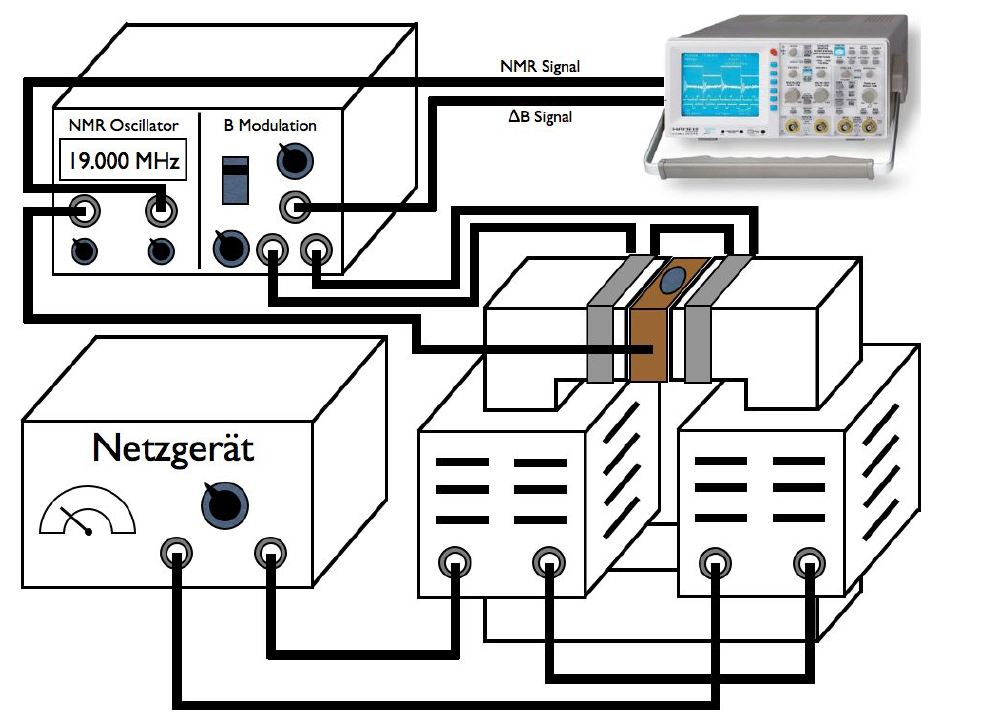
\includegraphics[scale=0.8]{Bild/Setup1}
	\centering
	\caption[Block Diagram for Setup 1]{Setup for measuring the resonance frequency with a sinus modulation.}
	\label{Exp_part1}
\end{figure}
\subsubsection{Lock-In Method}
For the second part the lock-in method is used since it is more precise duo to its lower background noise. Instead of the former absorption curve this method gives the differentiated curve. For the modulation of the magnetic field the superposition of a sinus and a sawtooth is used. Here the sawtooth is used mainly for the variance of the field while the sinus is used to create the differentiated signal since it has a similar frequency to the reference signal. The former minima of the absorption curve will now be the 'Nulldurchgang' of the signal. The moment the 'Nulldurchgang' of both measured signals overlap the correct resonance frequency is hit. Examples of both signals are shown in figure \ref{SägezahnBsp} and the setup is given in figure \ref{Exp_part2}.
\begin{figure}[ht]
	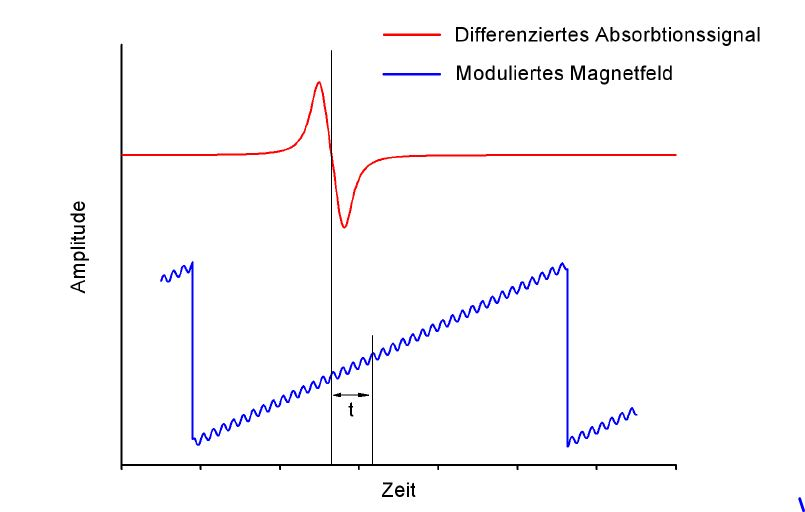
\includegraphics[scale=0.8]{Bild/BspLockIn}
	\centering
	\caption{Derived absorption signal in red. Superposition of sinus and sawtooth waves with both 'Nulldurchgängen' aligned.}
	\label{SägezahnBsp}
\end{figure}
\begin{figure}[ht]
	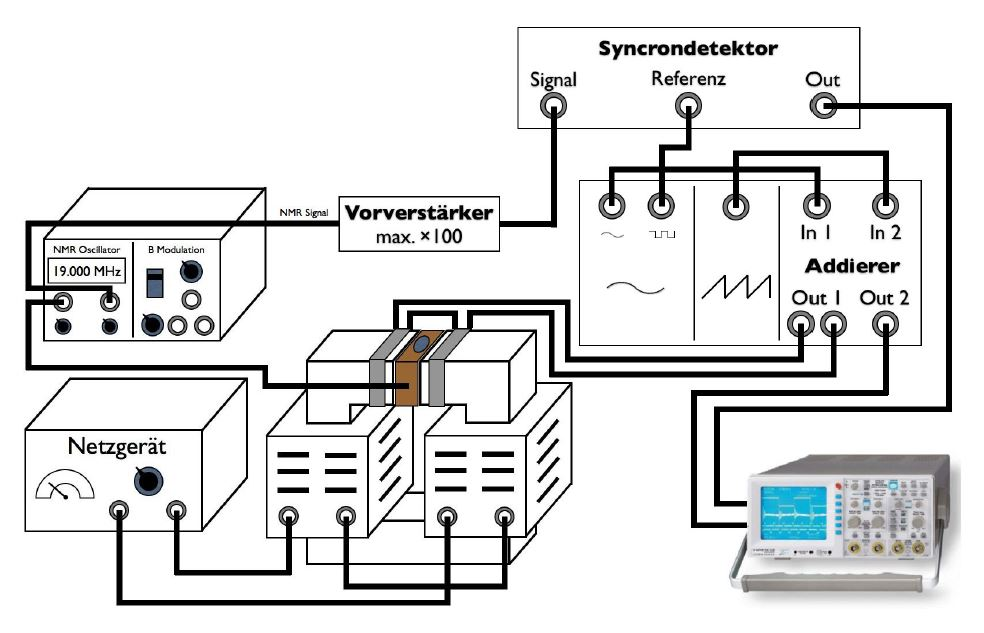
\includegraphics[scale=0.8]{Bild/Setup2}
	\centering
	\caption[Block Diagram for Setup 2]{Setup for measuring the resonance frequency with the lock-in method.}
	\label{Exp_part2}
\end{figure}


	\section{Durchführung des Versuches}
Vor der mündlichen Abfrage wurde die Messung vom Cobalt Spektrum mit dem CdTe Kristall gestartet mit einer Messzeit von einer Stunde. Nach der der mündlichen Abfrage wurde der CdTe Kristall gegen eine Silizium Diode getauscht und das zweite Cobalt Spektrum wurde mit der Messzeit von einer Stunde aufgenommen. \par
Während die obige Messung lief wurde mit den Vorbereitungen Absorptions- und Transmissionsmessungen zu Silizium gestartet. Es wurde der Strahlengang eingestellt und vorläufige Parameter des Lock-in Verstärkers gefunden.\par
Nun wurde auch das Cobalt Spektrum mittels der Silizium Diode aufgenommen, weshalb die Probe auf Americium gewechselt wurde und dessen Spektrum aufgezeichnet wurde. Die Messzeit betrug wieder eine Stunde.\par
Nach der ersten Testmessung zu Transmission und Absorption wurden die finalen Verstärkereinstellungen vorgenommen. Es wurden zwei normale Messungen und drei Untergrundmessungen aufgezeichnet: Eine ohne die Silizium Probe, eine ohne das Gitter und eine mit abgedunkeltem Spalt. Hierzu wurde das Gitter von $-90^{\circ}$ bis $+90^{\circ}$ gedreht und immer die Position des Gitters und der Widerstand der Probe sowie die Spannung des Pyrodetektors aufgezeichnet.\par
Nach Abschluss der ersten Americium Messung wurde klar, dass die Probe in der falschen Orientierung auf den Detektor platziert wurde, die Zählrate war viel niedriger als erwartet. Nachdem die Probe richtig platziert wurde, konnte die Messung mit Dauer einer Stunde erneut gestartet werden.\par
Da die Absorptions- und Transmissionsmessungen nun für Silizium abgeschlossen sind, wurde der Aufbau für die Germanium Probe vorbereitet: Das Gitter, der Filter und die Probe wurden vertauscht. Nun wurde der Verstärker für die Germanium Probe angepasst. Leider gab es zunächst Probleme, sodass man die realen Maxima erst bei maximaler Verstärkung finden konnte. Alls die Fehlersuche sich hinzog wurde beschlossen sich aufzuteilen und die Haynes und Shockley Messungen parallel durchzuführen.\par
Zunächst wurde der Offset von Glasfaser zu Elektrode bestimmt, anschließend wurde der Versuchsaufbau in Betrieb genommen. Es wurde nun die minimale Spannung  gefunden, bei welcher vermutet wurde, dass eine Auswertung der Messung in Form einer angepassten Gaußkurve möglich ist. Dann wurde in $2\,$V, später $4\,$V Schritten die Spannung erhöht bis zur maximal möglichen Spannung von $48\,$V.\par
Nun war die Messung des Americium Spektrums mit der Silizium Diode abgeschlossen und sie wurde gegen den CdTe Kristall getauscht. Anschließend wurde die letzte Messung gestartet. \par
Für das Haynes und Shockley Experiment wurden nun die Abstandsmessungen durchgeführt. Hierbei wurde zunächst die maximale Spannung an der Probe angelegt, und der Abstand so lange erhöht bis zur maximalen Distanz, bei welcher es für möglich gehalten wurde, eine Auswertung durchzuführen. Diese lag bei $9\,$mm auf der angebrachten Skala. Der Abstand wurde immer um einen mm zwischen den gespeicherten Messungen reduziert, bis zum minimalen Abstand von $2\,$mm. Es wurde nun noch einmal der Offset zwischen Glasfaser und Elektrode bestimmt, welcher jetzt $3.6\,$mm betrug. \par
Währenddessen wurde der Strahlenverlauf der Absorptions- und Transmissionsmessungen angepasst, sodass hier auch die oben erwähnten Messungen aufgenommen werden konnten.
	\section{Analysis}
\subsection{The Conductor Loops}
To calculate the $B_z$ value and the dipole moment $p$, there are two different way. The first one is to calculate the theoretical magnetic field as well as dipole moment by using the properties of the conductor loop and the applied voltage.\par
Here the equation \ref{Dipolmoment1} was used.
\begin{equation}
	p(R)=AI(R)=\pi r^2I(R)=\pi r^2 \frac{U}{R}
	\label{Dipolmoment1}
\end{equation}
The error is than computed using Gaussian error propagation by following equation:
\begin{equation}
	\sigma_p=\sqrt{\left(\frac{\pi U r \sigma_r}{R}\right)^2+\left(\frac{\pi r^2 \sigma_U}{R}\right)^2+\left(\frac{\pi r^2 U \sigma_R}{R^2}\right)^2}
\end{equation}
The diameter $d$ of the loop was measured multiples times and the mean was taken to get the radius . The error of the mean was calculated using equation \ref{Meanerror}. After this the value was divided by $2$ to get the radius.\par
\begin{equation}
	\sigma_x=\sqrt{\left(\frac{1}{n-1}\sum_{i=1}^{n}(x_i-\bar{x})^2\right)}
	\label{Meanerror}
\end{equation}
The voltage was gained by measuring the two attached batteries and adding them together. The values for the different resistors were given in the manual of the experiment\cite{anleitung} and are noted in table \ref{tableResi}.\par  
\begin{equation*}
	r = (1.558 \pm 0.010)\,mm
\end{equation*}
\begin{equation*}
	U_{ges} = U_1 + U_2 = (1.459\pm0.005 + 1.494\pm0.005)\,\text{V} = (2.9530\pm0.0007)\,\text{V}
\end{equation*}
\begin{table}[ht]
	\begin{Dtabular}[1.1]{|c|c|c|c|c|c|}
		\hline
		&Resistor 1&Resistor 2&Resistor 3&Resistor 4&Resistor 5\\
		\hline
		$\Omega$&$51.47\pm0.05$&$100.80\pm0.10$&$300.80\pm0.30$&$510.6\pm0.5$&$1000.0\pm1.0$\\
		\hline
	\end{Dtabular}
	\centering
	\caption[Resistors]{Different Resistors for the five conductor loop measurements.}
	\label{tableResi}
\end{table}
With this the dipole moment for the different Resistors was calculated and are written down in table \ref{Messwerte1}.\par
It can now be used to compute the magnetic field $B_z$ using equation \ref{DipolFeld}.
\begin{equation}
	B_z = \frac{\mu_0 p}{2\pi z^3}
	\label{DipolFeld}
\end{equation}
In this equation the value z is the distance of the probe to the SQUID. This was measured by measuring the length of the kryostat from top to the probe as well as from the top to the SQUID. The difference of both is the distance from probe to SQUID. To decrease the errors the mean of multiple distance measurements were taken.
\begin{equation*}
	z=(2.65 \pm 0.12)\,\text{cm}
\end{equation*}
The with that calculated value $B_z$ is also in table \ref{Messwerte1}.
\begin{table}[ht]
	\begin{Dtabular}[1.1]{|c|c|c|}
		\hline
		&$p$\,[Am$^2$]&$B_z$\,[T]\\
		\hline
		R1&$\left(8.75 \pm 0.11\right) \times 10^{-7} $&$\left(9.4 \pm 1.2\right) \times 10^{-9}$\\
		\hline
		R2&$\left(4.47 \pm 0.06\right) \times 10^{-7} $&$\left(4.8 \pm 0.6\right) \times 10^{-9}$\\
		\hline
		R3&$\left(1.498 \pm 0.020\right) \times 10^{-7}$ &$\left(1.61 \pm 0.21\right) \times 10^{-9}$\\
		\hline
		R4&$\left(8.82 \pm 0.12\right) \times 10^{-8} $&$\left(9.5 \pm 1.2\right) \times 10^{-10}$\\
		\hline
		R5&$\left(4.51 \pm 0.06\right) \times 10^{-8}$ &$\left(4.8 \pm 0.6\right) \times 10^{-10}$\\ 
		\hline
		
	\end{Dtabular}
	\centering
	\caption[Values of Dipole Moment and Magnetic Field]{Values of the magnetic field and the dipole moment for the five different resistors. Calculated by using equation \ref{Dipolmoment1} and \ref{DipolFeld}}
	\label{Messwerte1}
\end{table} 
\newpage
The other way to calculate the dipole moment and magnetic field was by using the measured signals of the SQUID. Here the signal shapes were fitted with the help of Pythons package  \verb|scipy.optimize| with the method \verb|curve_fit|. Here the form given in equation \ref{Sinusfit} was used. With that the offset $a$, the frequency $\omega=c$ as well as the amplitude $b=\Delta V$ can be calculated. 
\begin{equation}
	f(x)=a+b\sin(cx+d)
	\label{Sinusfit}
\end{equation}
An example of the fits can be seen in figure \ref{Fit1} the other ones are in the appendix.\par
The parameters $b$ of the different measurements for each resistor were taken and the weighted mean of them was taken. For this mean the equation \ref{WMean} and \ref{Er_WMean} were used. The values are listed in table \ref{Messwerte2}. \par
\begin{equation}
	\bar{x}_g=\frac{\sum_ig_ix_i}{\sum_ig_i} \qquad \text{with} \qquad g_i=\frac{1}{\sigma_i^2}
	\label{WMean}
\end{equation}
\begin{equation}
	\sigma_{\bar{x}_g}=\frac{1}{\sqrt{\sum_i\nicefrac{1}{\sigma_i^2}}}
	\label{Er_WMean}
\end{equation}
With these voltages the magnetic field $B_z$ can be computed using equation \ref{Bz}. An similar to the calculation for the theoretical values equation \ref{DipolFeld} can be used to gain the dipole moment $p$.
\begin{equation}
	B_z=F\frac{\Delta V}{s_i}
	\label{Bz}
\end{equation}
The value of $F$ the field flux coefficient is $9.3\,\frac{\text{nT}}{\Phi_0}$ and $s_i$ is transfer coefficient. This one can be looked up in the manual\cite{anleitung}. For the conductor loops a FB-R resistance of $100$\,k$\Omega$ was chosen which leads to a $s_i$ value of $1900\,\frac{mV}{\Phi_0}$. The values of the calculated magnetic field and dipole moment are noted in table \ref{Messwerte2}
\begin{table}[ht]
	\begin{Dtabular}[1.1]{|c|c|c|c|}
		\hline
		&$p$[Am$^2$]&$B_z$[T]&$\Delta V$\,[V]\\
		\hline
		R1&$\left(2.19 \pm 0.29\right) \times 10^{-7} $&$\left(2.356 \pm 0.007\right) \times 10^{-9} $&$0.2407 \pm 0.0007$\\
		\hline
		R2&$\left(1.18 \pm 0.15\right) \times 10^{-7} $&$\left(1.271 \pm 0.007\right) \times 10^{-9} $&$0.1298 \pm 0.0007$\\
		\hline
		R3&$\left(3.9 \pm 0.5\right) \times 10^{-8} $&$\left(4.17 \pm 0.08\right) \times 10^{-10} $&$0.0426 \pm 0.0008$\\
		\hline
		R4&$\left(2.36 \pm 0.31\right) \times 10^{-8}$&$\left(2.54 \pm 0.05\right) \times 10^{-10}$&$0.0259 \pm 0.0005$\\
		\hline
		R5&$\left(1.37 \pm 0.19\right) \times 10^{-8} $&$\left(1.47 \pm 0.06\right) \times 10^{-10}$&$0.0150 \pm 0.0006$\\
		\hline
	\end{Dtabular}
	\centering
	\caption[Values of the Loops with the Fit Method]{Measured values for the different conductor loops using the fits of the SQUID signals.}
	\label{Messwerte2}
\end{table}
\begin{figure}[ht]
	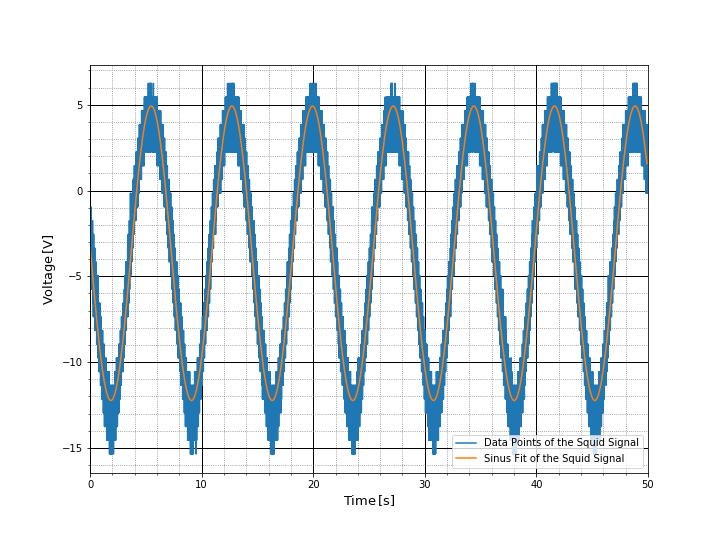
\includegraphics[scale=0.5]{Bild/r1_5_2}
	\centering
	\caption[Example of the Data Plots with SInus Fit]{In blue the signal coming from the SQUID and in orange the sinus fit to the data points.}
\end{figure}
\FloatBarrier
\subsection{Other Samples}
During the measurement other samples were tested with the SQUID. The SQUID signals were analysed in a similar way to the conductor Loops before. The sinus of the form \ref{Sinusfit} was fitted on the signal. The mean of amplitude which is parameter $b$ was computed for the different samples and with this the magnetic field $B_z$ and dipole moment could be calculated and can be found in table \ref{Messwerte3} in the table below.\par
\begin{table}[ht]
	\begin{Dtabular}[1.1]{|c|c|c|c|}
		\hline
		&$p$[Am$^2$]&$B_z$[T]&$\Delta V$\,[V]\\
		\hline
		Iron chips&$\left(1.84 \pm 0.25\right) \times 10^{-8}  $&$\left(1.98 \pm 0.07\right) \times 10^{-10}  $&$0.0202 \pm 0.0007 $\\
		\hline
		Gold lamella&$ \left(3.2 \pm 0.4\right) \times 10^{-8} $&$ \left(3.42 \pm 0.12\right) \times 10^{-10} $&$0.0349 \pm 0.0012 $\\
		\hline
		Magnet chips&$\left(7.8 \pm 1.0\right) \times 10^{-6}  $&$\left(8.408 \pm 0.030\right) \times 10^{-8}  $&$8.589 \pm 0.031 $\\
		\hline
		Stone&$\left(7.4 \pm 1.1\right) \times 10^{-10}  $&$ \left(7.9 \pm 0.5\right) \times 10^{-12} $&$ 0.00081 \pm 0.00005$\\
		\hline
		Magnet&$0.000262 \pm 0.000034 $&$\left(2.814 \pm 0.014\right) \times 10^{-6}  $&$6.355 \pm 0.031 $\\
		\hline
	\end{Dtabular}
	\centering
	\caption[Values of the Samples with the Fit Method]{Measured and calculated values for different materials and forms of samples.}
	\label{Messwerte3}
\end{table}
\subsection{Polar Representation}
For the samples and conductor loops the polar representation should be plotted. For this one period of the data points was taken. With the help of the coordinate transformation of the manual\cite{anleitung}:
\begin{equation}
	x_i=|B_z|\cdot \cos(\alpha)
\end{equation}
\begin{equation}
	y_i=|B_z|\cdot \sin(\alpha)
\end{equation}
Here $\alpha$ is the rotation angle. For the stone the polar representation can be seen in figure \ref{Stone}, the rest is in the appendix.
\begin{figure}[ht]
	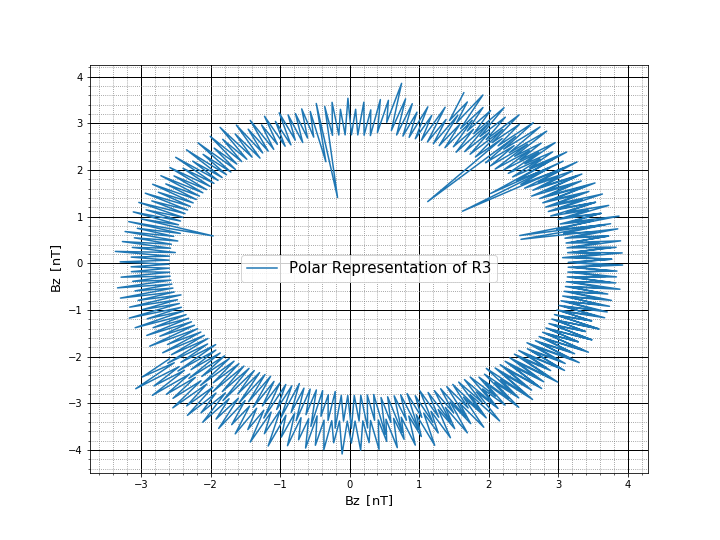
\includegraphics[scale=0.5]{Bild/R3}
	\centering
	\caption[Polar Representation for R2 Conductor Loop]{Polar Representation for one period of the signal coming from the R2 Conductor Loop.}
\end{figure}\\	
	\section{Zusammenfassung}
Wenn man die gemessenen Werte mit denen des Literatur Wertes von $119\,$ns mit der Formel \ref{Vergleich} vergleicht erhält man die in Tabelle \ref{VglTable} beschriebenen Werte. \\
\begin{table}
	\begin{Dtabular}[1.1]{|c|c|c|}
		\hline
		Messreihe&Lebensdauer $\tau$[ns]&Vergleichswert\\
		\hline
		Abkühlen 1 bei $0^\circ$&$(1.224\pm0.022)$&\\
		\hline
		Abkühlen 1 bei $90^\circ$&&\\
		\hline
		Aufwärmen bei $0^\circ$&&\\
		\hline
		Abkühlen 2 bei $0^\circ$&&\\
		\hline
		Abkühlen 2 bei $90^\circ$&&\\
		\hline
	\end{Dtabular}
\end{table}
Man erkennt schnell, dass alle gemessenen Werte bis auf die Aufwärmmessung mit dem Literaturwert kompatibel sind. Die große Diskrepanz kann man dadurch erklären, dass für die Messung während des Aufwärmvorgangs nicht gewartet wurde bis die Temperatur des Thermometers mit der der Probe angeglichen hat. Dadurch ziehen wir einen großen systematischen Fehler mit welcher die Unverträglichkeit erklären könnte. \par Ein weiteres Problem ist sicher die geringe Anzahl an Messpunkten die wir in allen Messreihen hatten, wodurch sich natürlich unsere Messreihe verschlechtert. 
	
	
	
	
	
	\section{Tabellen}
	\listoftables
	\section{Bilder}
	\listoffigures
	\section{Bibliograpy}
	\bibliographystyle{plain}
	\bibliography{Quellen}
	\addcontentsline{toc}{section}{Literatur}
	\section{Anhang}
	\begin{figure}
	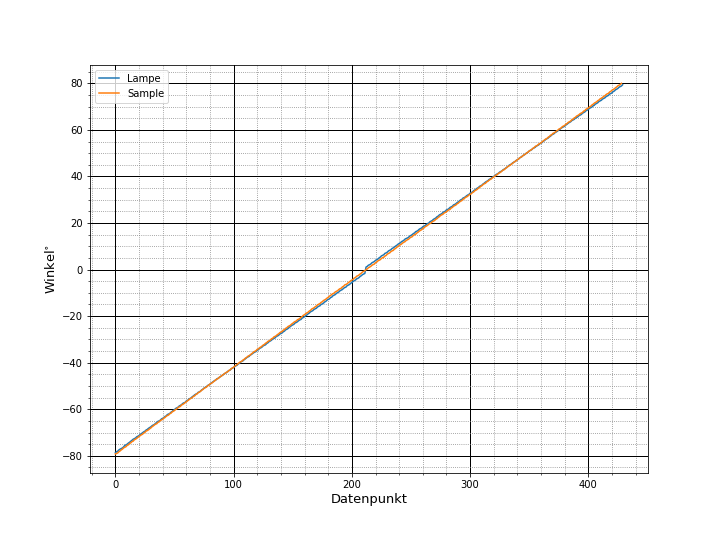
\includegraphics[scale=0.5]{Bilder/anhang/korrektur_channels_2}
	\centering
	\caption[Korrigierter Lampendatensatz 2. Silizium messung]{\small Auftragung der gemessenen Winkel für die Lampenmessung und erste Silizium Messung nach der Korrektur. Beide stimmen in den relevanten Bereichen bei ca. $30^{\circ}-40^{\circ}$ weitgehend überein.}
\end{figure}
\begin{figure}
	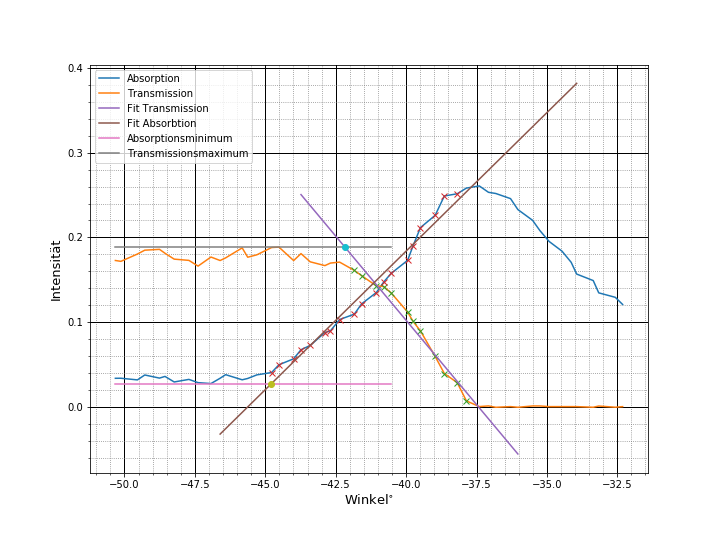
\includegraphics[scale=0.5]{Bilder/anhang/si_2_l}
	\centering
	\caption[Geraden Anpassungen 2. Silizium Messung links]{\small Auftragung von Intensität der normalisierten Datenreihen gegen die  Winkel in der Nähe der Stelle Gleichwahrscheinlicher Absorption und Transmission bei Winkeln kleiner als $0^\circ$. Es sind zusätzlich die angepassten Geraden zur Absorption und Transmission eingezeichnet. Die Horizontalen wurden durch die Maxima der dahinterliegenden Datenpunkte bestimmt. Die Schnittpunkte der Geraden mit ihren jeweiligen Horizontalen sind auch eingezeichnet.}
\end{figure}
\begin{figure}
	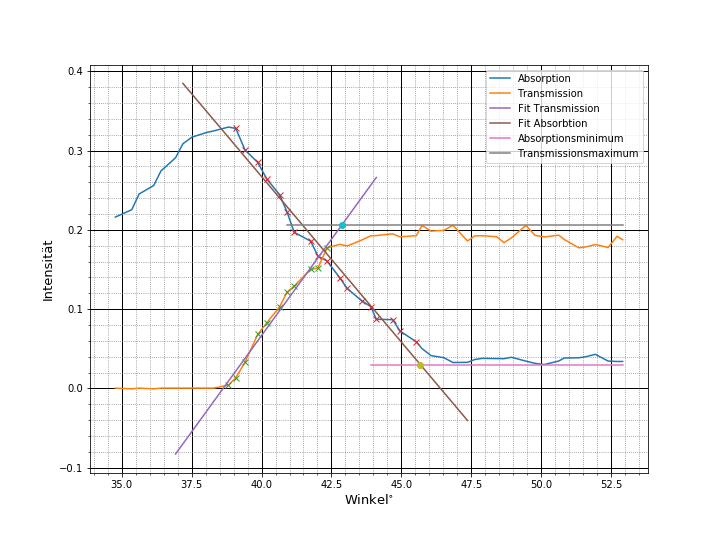
\includegraphics[scale=0.5]{Bilder/anhang/si_2_r}
	\centering
	\caption[Geraden Anpassungen 2. Silizium Messung rechts]{\small Auftragung von Intensität der normalisierten Datenreihen gegen die  Winkel der zweiten Silizium Messung in der Nähe der Stelle Gleichwahrscheinlicher Absorption und Transmission bei Winkeln größer als $0^\circ$. Es sind zusätzlich die angepassten Geraden zur Absorption und Transmission eingezeichnet. Die Horizontalen wurden durch die Maxima der dahinterliegenden Datenpunkte bestimmt. Die Schnittpunkte der Geraden mit ihren jeweiligen Horizontalen sind auch eingezeichnet.}
	\label{si_2_r}
\end{figure}
\begin{figure}
	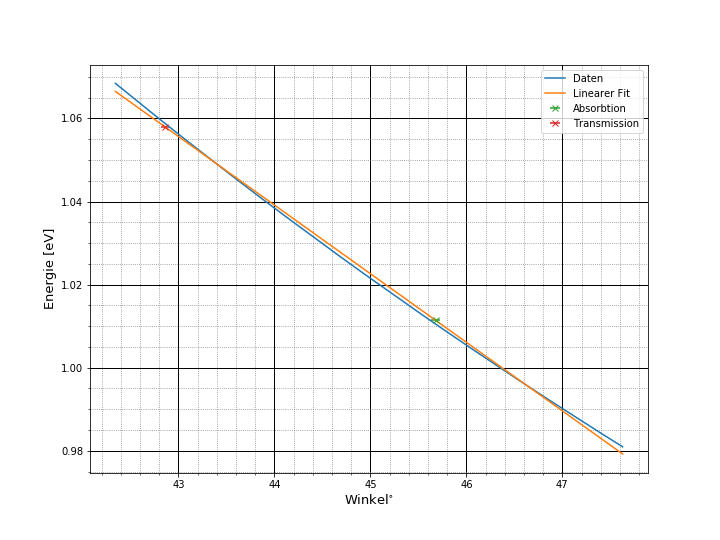
\includegraphics[scale=0.5]{Bilder/anhang/si_2_l_energie}
	\centering
	\caption[Energiebestimmung 2. Si Messung links]{\small Auftragung der Energie gegen den Winkel der zweiten Silizium Messung. Die angepasste Gerade und die beiden Schnittpunkte sind auch eingetragen.}
\end{figure}
\begin{figure}
	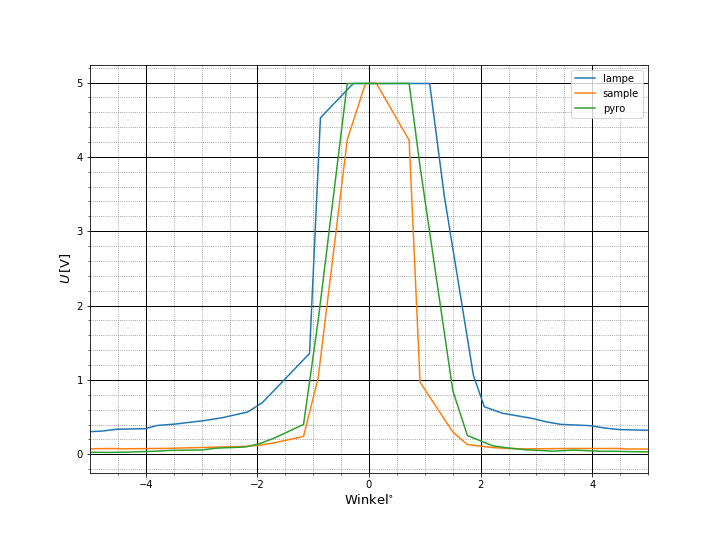
\includegraphics[scale=0.5]{Bilder/anhang/winkelkorrektur_vorher}
	\centering
	\caption[Mittelpunkt der 2. Si Messung vor Winkelkorrektur]{\small Auftragung der Intensität gegen den Winkel der zweiten Silizium Messung in der Nähe von $0^\circ$ vor der Korrektur.}
\end{figure}
\begin{figure}
	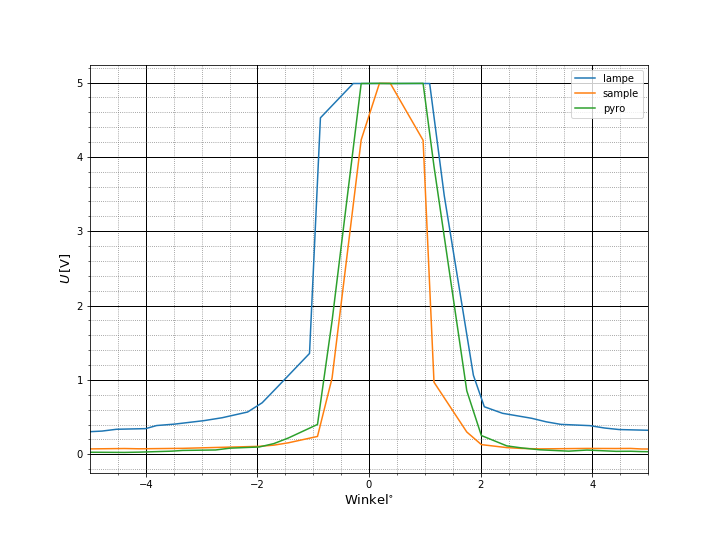
\includegraphics[scale=0.5]{Bilder/anhang/winkelkorrektur_nachher}
	\centering
	\caption[Mittelpunkt der 2. Si Messung vor Winkelkorrektur]{\small Auftragung der Intensität gegen den Winkel der zweiten Silizium Messung in der Nähe von $0^\circ$ nach der Korrektur.}
\end{figure}
\begin{figure}
	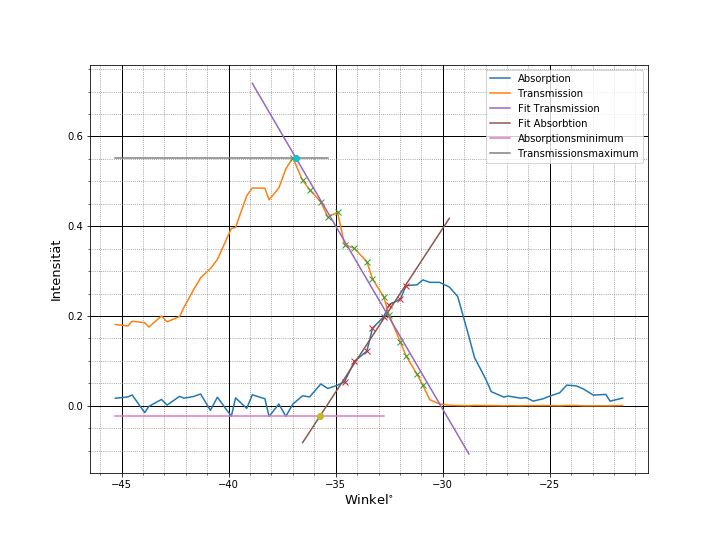
\includegraphics[scale=0.5]{Bilder/anhang/ge_r}
	\caption[Geraden Anpassungen Germanium Messung links]{\small Auftragung von Intensität der normalisierten Datenreihen von Germanium gegen die  Winkel in der Nähe der Stelle Gleichwahrscheinlicher Absorption und Transmission bei Winkeln größer als $0^\circ$. Es sind zusätzlich die angepassten Geraden zur Absorption und Transmission eingezeichnet. Die Horizontalen wurden durch die Maxima der dahinterliegenden Datenpunkte bestimmt. Die Schnittpunkte der Geraden mit ihren jeweiligen Horizontalen sind auch eingezeichnet.}
\end{figure}
\begin{figure}
	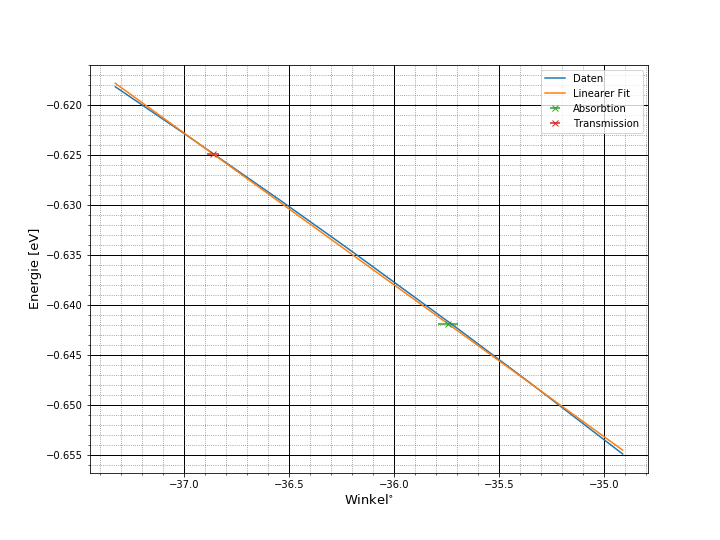
\includegraphics[scale=0.5]{Bilder/anhang/ge_l_energie}
	\centering
	\caption[Energiebestimmung Ge Messung links]{\small Auftragung der Energie gegen den Winkel der Germanium Messung. Die angepasste Gerade und die beiden Schnittpunkte sind auch eingetragen.}
\end{figure}


\begin{figure}
	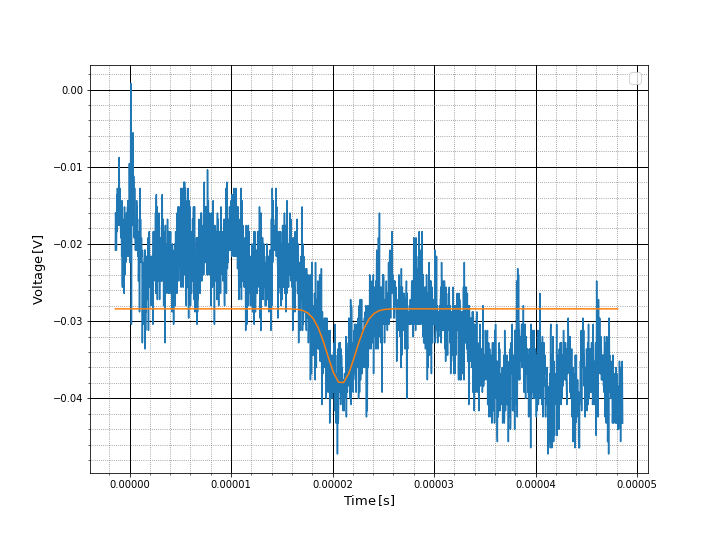
\includegraphics[scale=0.5]{Bild/S1}
	\centering
	\caption[Gaußfit an Messung bei Konst. Spannung 1]{Gaußfit an die Messungen der Elektronenwolken bei einer Spannung von $48\,$V und einem Abstand zwischen Nadel und Lase von $10.6$\,mm.}
\end{figure}
\begin{figure}
	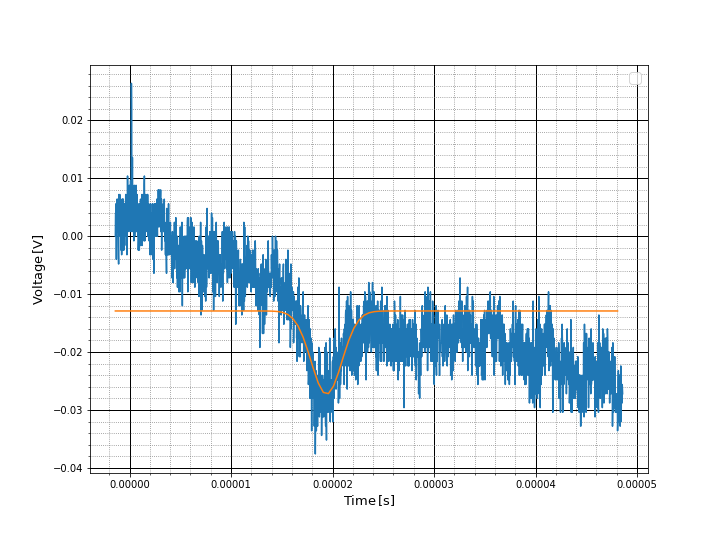
\includegraphics[scale=0.5]{Bild/S2}
	\centering
	\caption[Gaußfit an Messung bei Konst. Spannung 2]{Gaußfit an die Messungen der Elektronenwolken bei einer Spannung von $48\,$V und einem Abstand zwischen Nadel und Lase von $9.6$\,mm.}
\end{figure}
\begin{figure}
	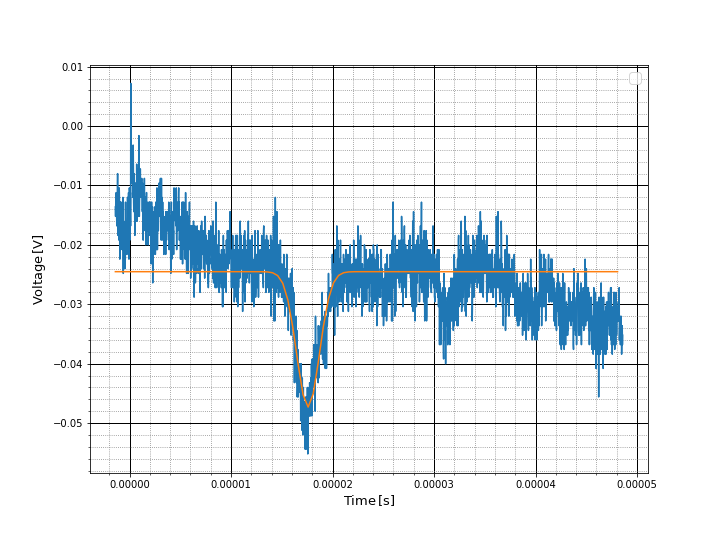
\includegraphics[scale=0.5]{Bild/S3}
	\centering
	\caption[Gaußfit an Messung bei Konst. Spannung 3]{Gaußfit an die Messungen der Elektronenwolken bei  einer Spannung von $48\,$V und einem Abstand zwischen Nadel und Lase von $8.6$\,mm.}
\end{figure}
\begin{figure}
	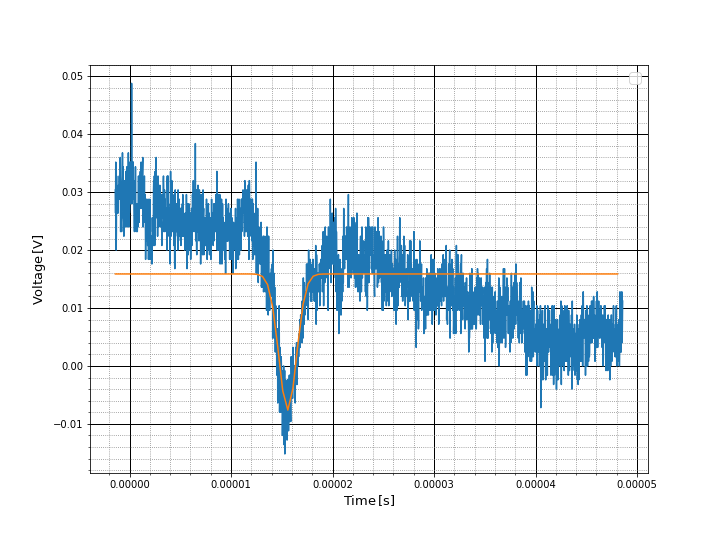
\includegraphics[scale=0.5]{Bild/S4}
	\centering
	\caption[Gaußfit an Messung bei Konst. Spannung 4]{Gaußfit an die Messungen der Elektronenwolken bei  einer Spannung von $48\,$V und einem Abstand zwischen Nadel und Lase von $7.6$\,mm.}
\end{figure}
\begin{figure}
	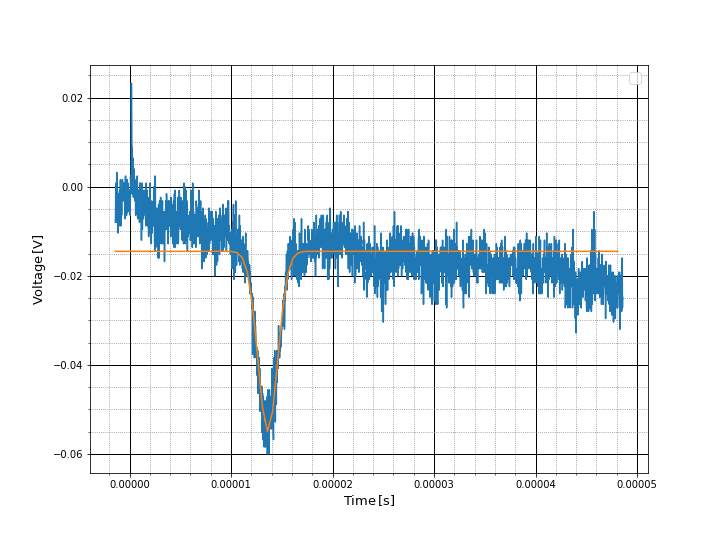
\includegraphics[scale=0.5]{Bild/S5}
	\centering
	\caption[Gaußfit an Messung bei Konst. Spannung 5]{Gaußfit an die Messungen der Elektronenwolken bei einer Spannung von $48\,$V und einem Abstand zwischen Nadel und Lase von $6.6$\,mm.}
\end{figure}
\begin{figure}
	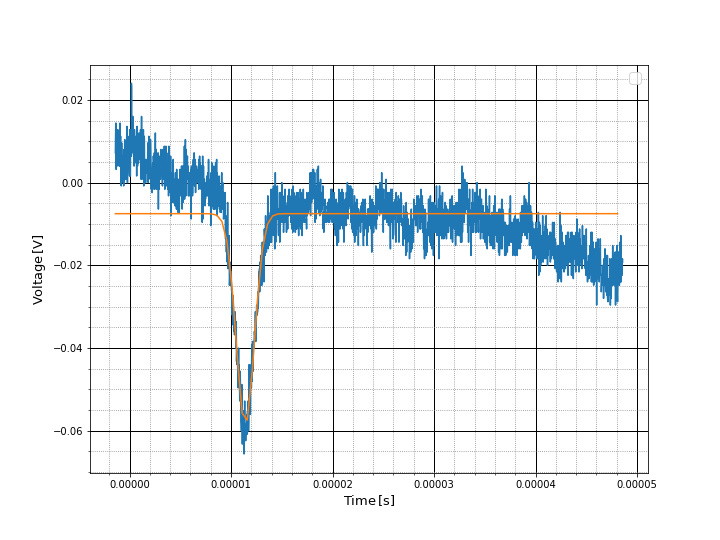
\includegraphics[scale=0.5]{Bild/S6}
	\centering
	\caption[Gaußfit an Messung bei Konst. Spannung 6]{Gaußfit an die Messungen der Elektronenwolken bei einer Spannung von $48\,$V und einem Abstand zwischen Nadel und Lase von $5.6$\,mm.}
\end{figure}
\begin{figure}
	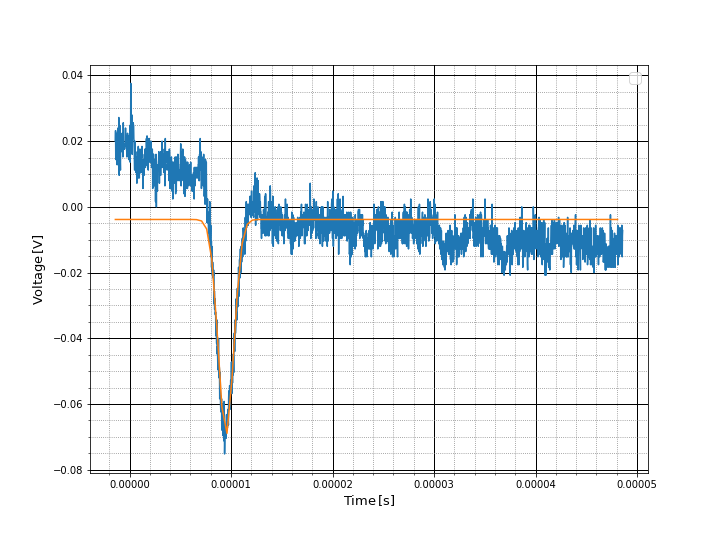
\includegraphics[scale=0.5]{Bild/S7}
	\centering
	\caption[Gaußfit an Messung bei Konst. Spannung 7]{Gaußfit an die Messungen der Elektronenwolken bei einer Spannung von $48\,$V und einem Abstand zwischen Nadel und Lase von $4.6$\,mm.}
\end{figure}
\begin{figure}
	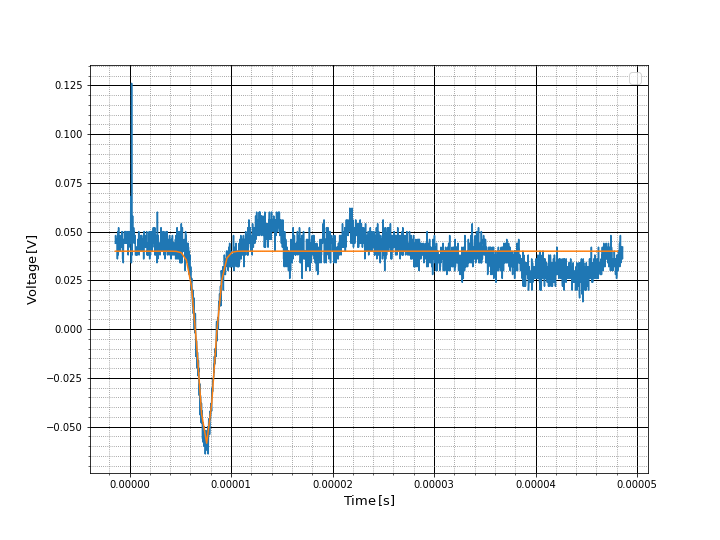
\includegraphics[scale=0.5]{Bild/S8}
	\centering
	\caption[Gaußfit an Messung bei Konst. Spannung 8]{Gaußfit an die Messungen der Elektronenwolken bei einer Spannung von $48\,$V und einem Abstand zwischen Nadel und Lase von $3.6$\,mm.}
\end{figure}

%Andere Messreihe

\begin{figure}
	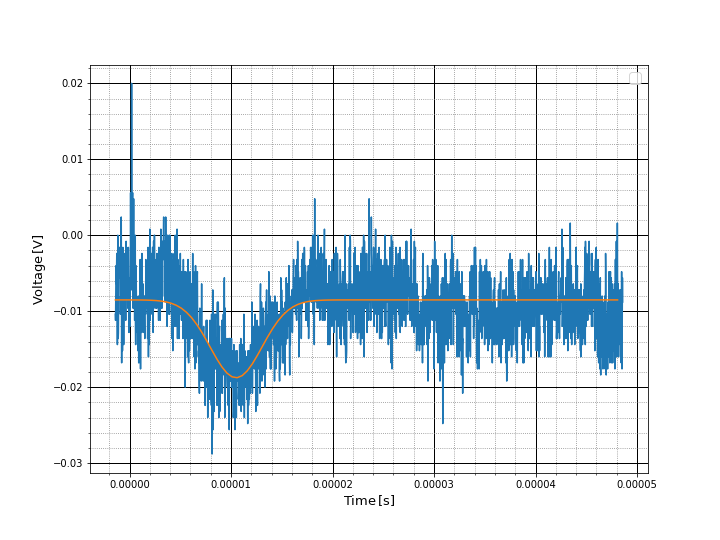
\includegraphics[scale=0.5]{Bild/A1}
	\centering
	\caption[Gaußfit an Messung bei Konst. Abstand]{Gaußfit an die Messungen der Elektronenwolken bei Konstantem Abstand von $3.6$\,mm und einer Spannung von $-13.2$\,V}
\end{figure}
\begin{figure}
	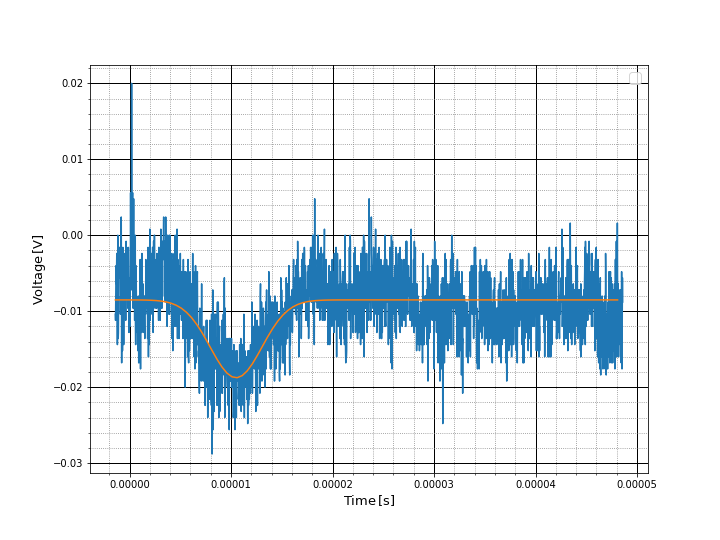
\includegraphics[scale=0.5]{Bild/A1}
	\centering
	\caption[Gaußfit an Messung bei Konst. Abstand]{Gaußfit an die Messungen der Elektronenwolken bei Konstantem Abstand von $3.6$\,mm und einer Spannung von $-15.2$\,V}
\end{figure}
\begin{figure}
	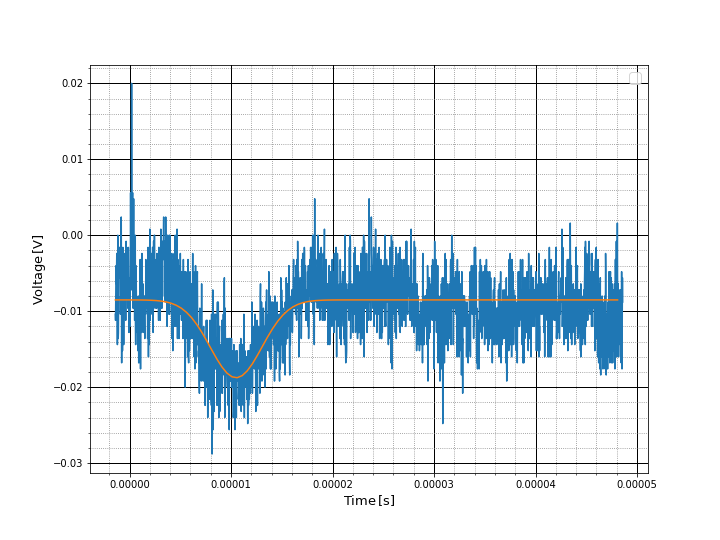
\includegraphics[scale=0.5]{Bild/A1}
	\centering
	\caption[Gaußfit an Messung bei Konst. Abstand]{Gaußfit an die Messungen der Elektronenwolken bei Konstantem Abstand von $3.6$\,mm und einer Spannung von $-18.4$\,V}
\end{figure}
\begin{figure}
	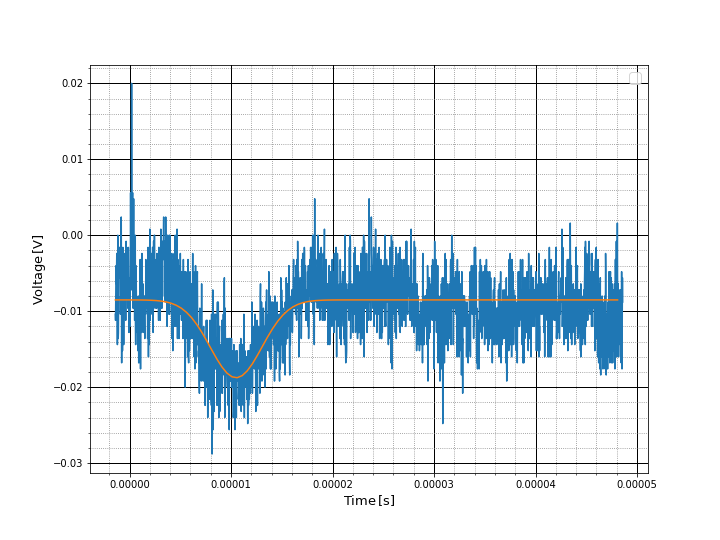
\includegraphics[scale=0.5]{Bild/A1}
	\centering
	\caption[Gaußfit an Messung bei Konst. Abstand]{Gaußfit an die Messungen der Elektronenwolken bei Konstantem Abstand von $3.6$\,mm und einer Spannung von $-20.4$\,V}
\end{figure}
\begin{figure}
	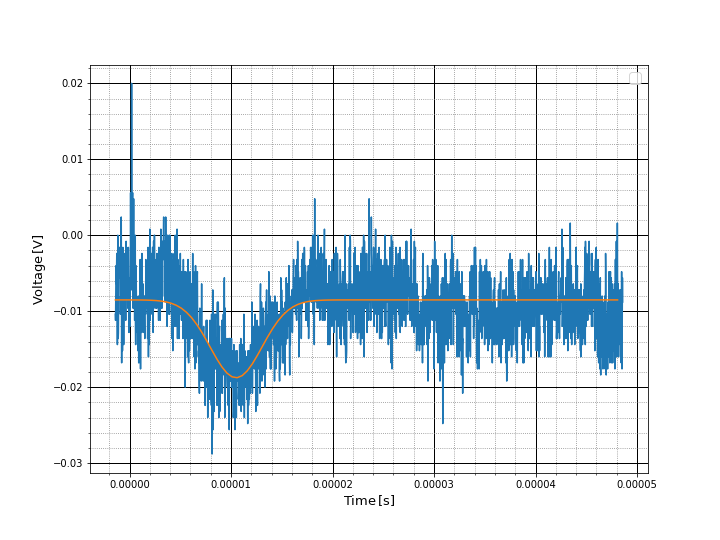
\includegraphics[scale=0.5]{Bild/A1}
	\centering
	\caption[Gaußfit an Messung bei Konst. Abstand]{Gaußfit an die Messungen der Elektronenwolken bei Konstantem Abstand von $3.6$\,mm und einer Spannung von $-22.4$\,V}
\end{figure}
\begin{figure}
	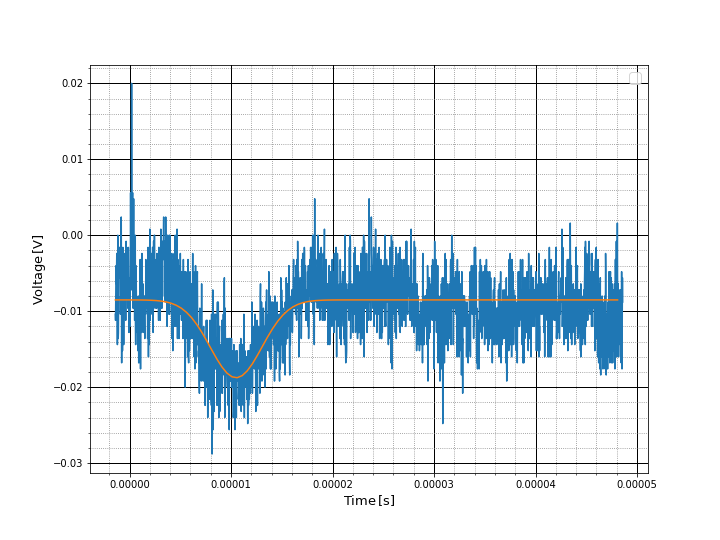
\includegraphics[scale=0.5]{Bild/A1}
	\centering
	\caption[Gaußfit an Messung bei Konst. Abstand]{Gaußfit an die Messungen der Elektronenwolken bei Konstantem Abstand von $3.6$\,mm und einer Spannung von $-24.4$\,V}
\end{figure}
\begin{figure}
	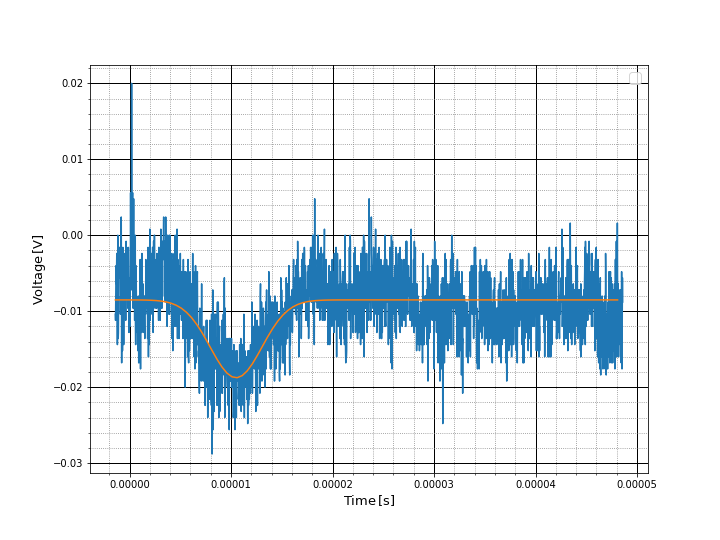
\includegraphics[scale=0.5]{Bild/A1}
	\centering
	\caption[Gaußfit an Messung bei Konst. Abstand]{Gaußfit an die Messungen der Elektronenwolken bei Konstantem Abstand von $3.6$\,mm und einer Spannung von $-28.0$\,V}
\end{figure}
\begin{figure}
	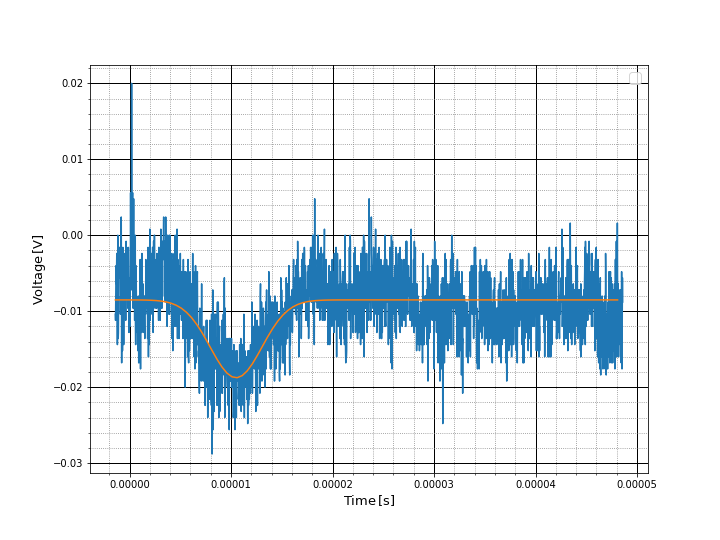
\includegraphics[scale=0.5]{Bild/A1}
	\centering
	\caption[Gaußfit an Messung bei Konst. Abstand]{Gaußfit an die Messungen der Elektronenwolken bei Konstantem Abstand von $3.6$\,mm und einer Spannung von $-32.0$\,V}
\end{figure}
\begin{figure}
	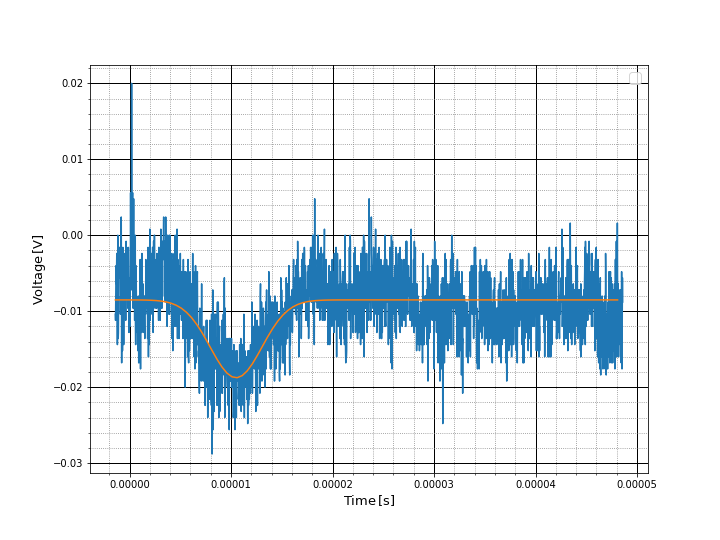
\includegraphics[scale=0.5]{Bild/A1}
	\centering
	\caption[Gaußfit an Messung bei Konst. Abstand]{Gaußfit an die Messungen der Elektronenwolken bei Konstantem Abstand von $3.6$\,mm und einer Spannung von $-36.0$\,V}
\end{figure}
\begin{figure}
	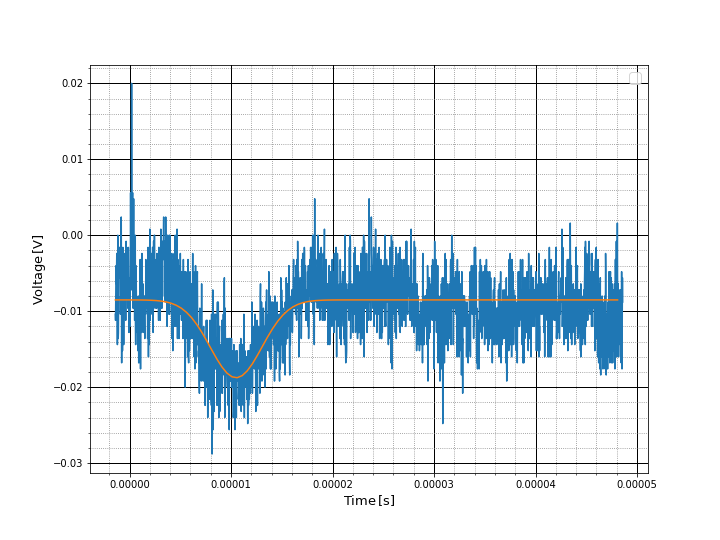
\includegraphics[scale=0.5]{Bild/A1}
	\centering
	\caption[Gaußfit an Messung bei Konst. Abstand]{Gaußfit an die Messungen der Elektronenwolken bei Konstantem Abstand von $3.6$\,mm und einer Spannung von $-40.0$\,V}
\end{figure}
\begin{figure}
	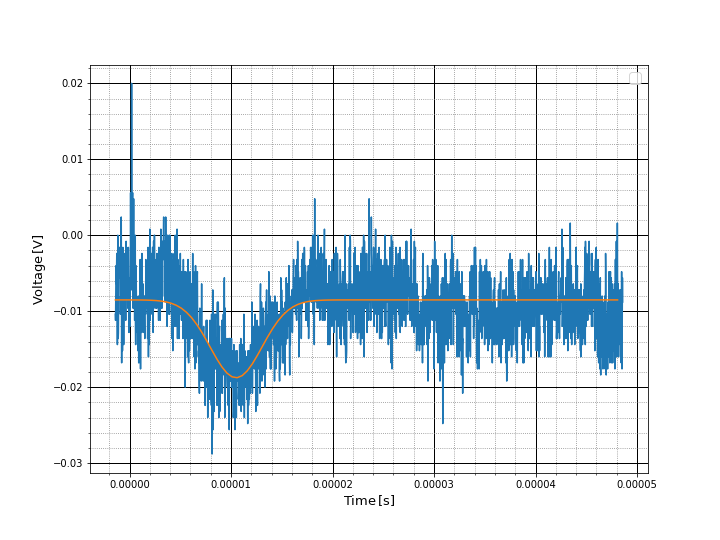
\includegraphics[scale=0.5]{Bild/A1}
	\centering
	\caption[Gaußfit an Messung bei Konst. Abstand]{Gaußfit an die Messungen der Elektronenwolken bei Konstantem Abstand von $3.6$\,mm und einer Spannung von $-44.0$\,V}
\end{figure}
\begin{figure}
	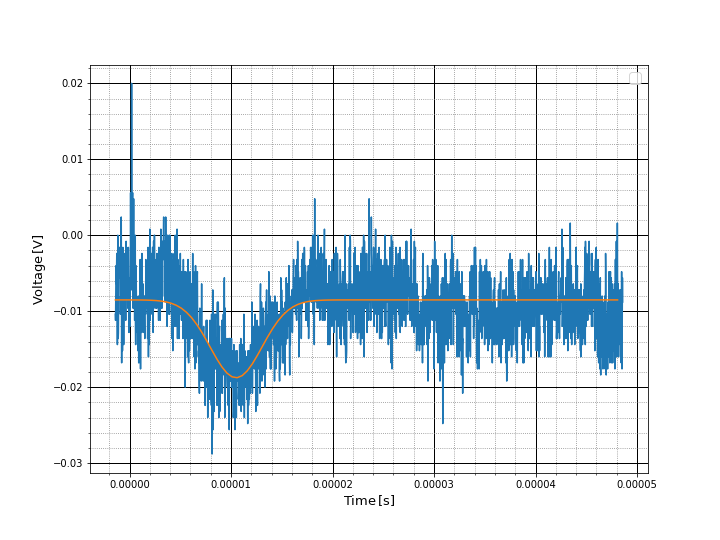
\includegraphics[scale=0.5]{Bild/A1}
	\centering
	\caption[Gaußfit an Messung bei Konst. Abstand]{Gaußfit an die Messungen der Elektronenwolken bei Konstantem Abstand von $3.6$\,mm und einer Spannung von $-46.0$\,V}
\end{figure}
\begin{figure}
	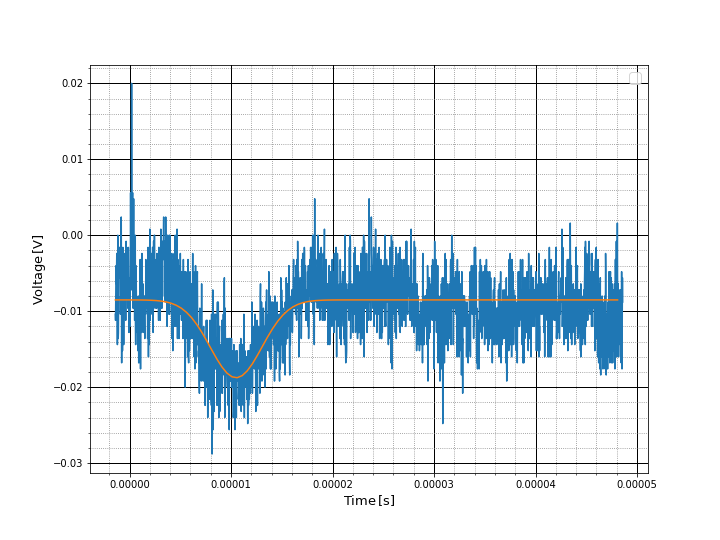
\includegraphics[scale=0.5]{Bild/A1}
	\centering
	\caption[Gaußfit an Messung bei Konst. Abstand]{Gaußfit an die Messungen der Elektronenwolken bei Konstantem Abstand von $3.6$\,mm und einer Spannung von $-48.0$\,V}
\end{figure}

%Lange Messungen

\begin{figure}[ht]
	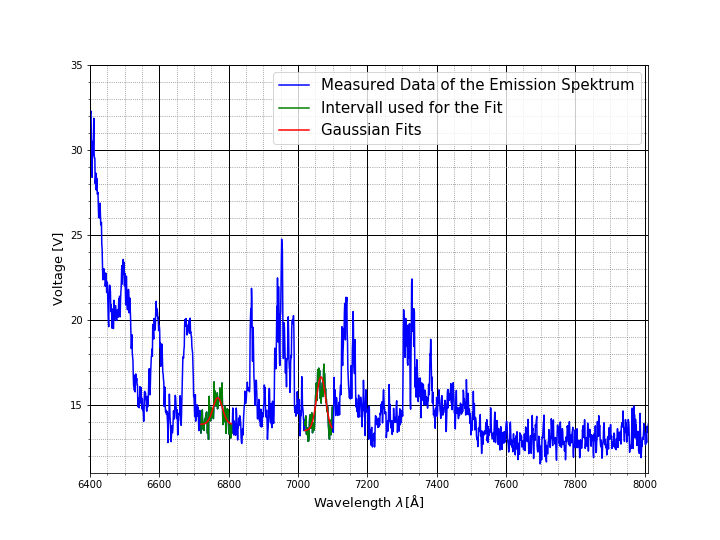
\includegraphics[scale=0.5]{Bild/ASg}
	\centering
	\caption{Gesamtes Spektrum von Americium mit Silizium aufgenommen.}
\end{figure}
\begin{figure}[ht]
	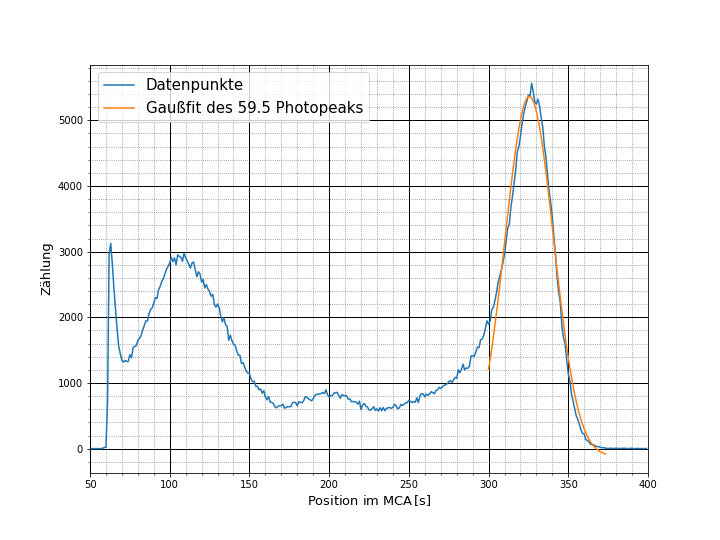
\includegraphics[scale=0.5]{Bild/ACg}
	\centering
	\caption{Gesamtes Spektrum von Americium mit CdTe aufgenommen.}
\end{figure}
\begin{figure}[ht]
	\includegraphics[scale=0.5]{Bild/CSg}
	\centering
	\caption{Gesamtes Spektrum von Cobalt mit Silizium aufgenommen.}
\end{figure}
\begin{figure}[ht]
	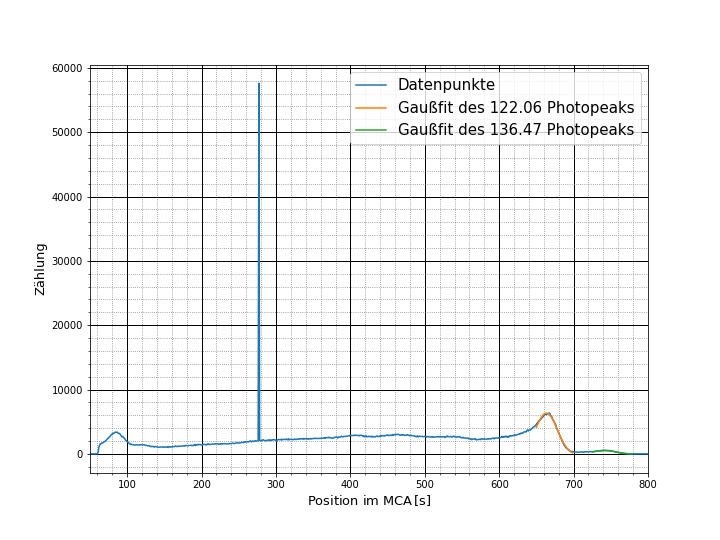
\includegraphics[scale=0.5]{Bild/CCg}
	\centering
	\caption{Gesamtes Spektrum von Cobalt mit CdTe aufgenommen.}
\end{figure}
\subsection{Laborbuch}
%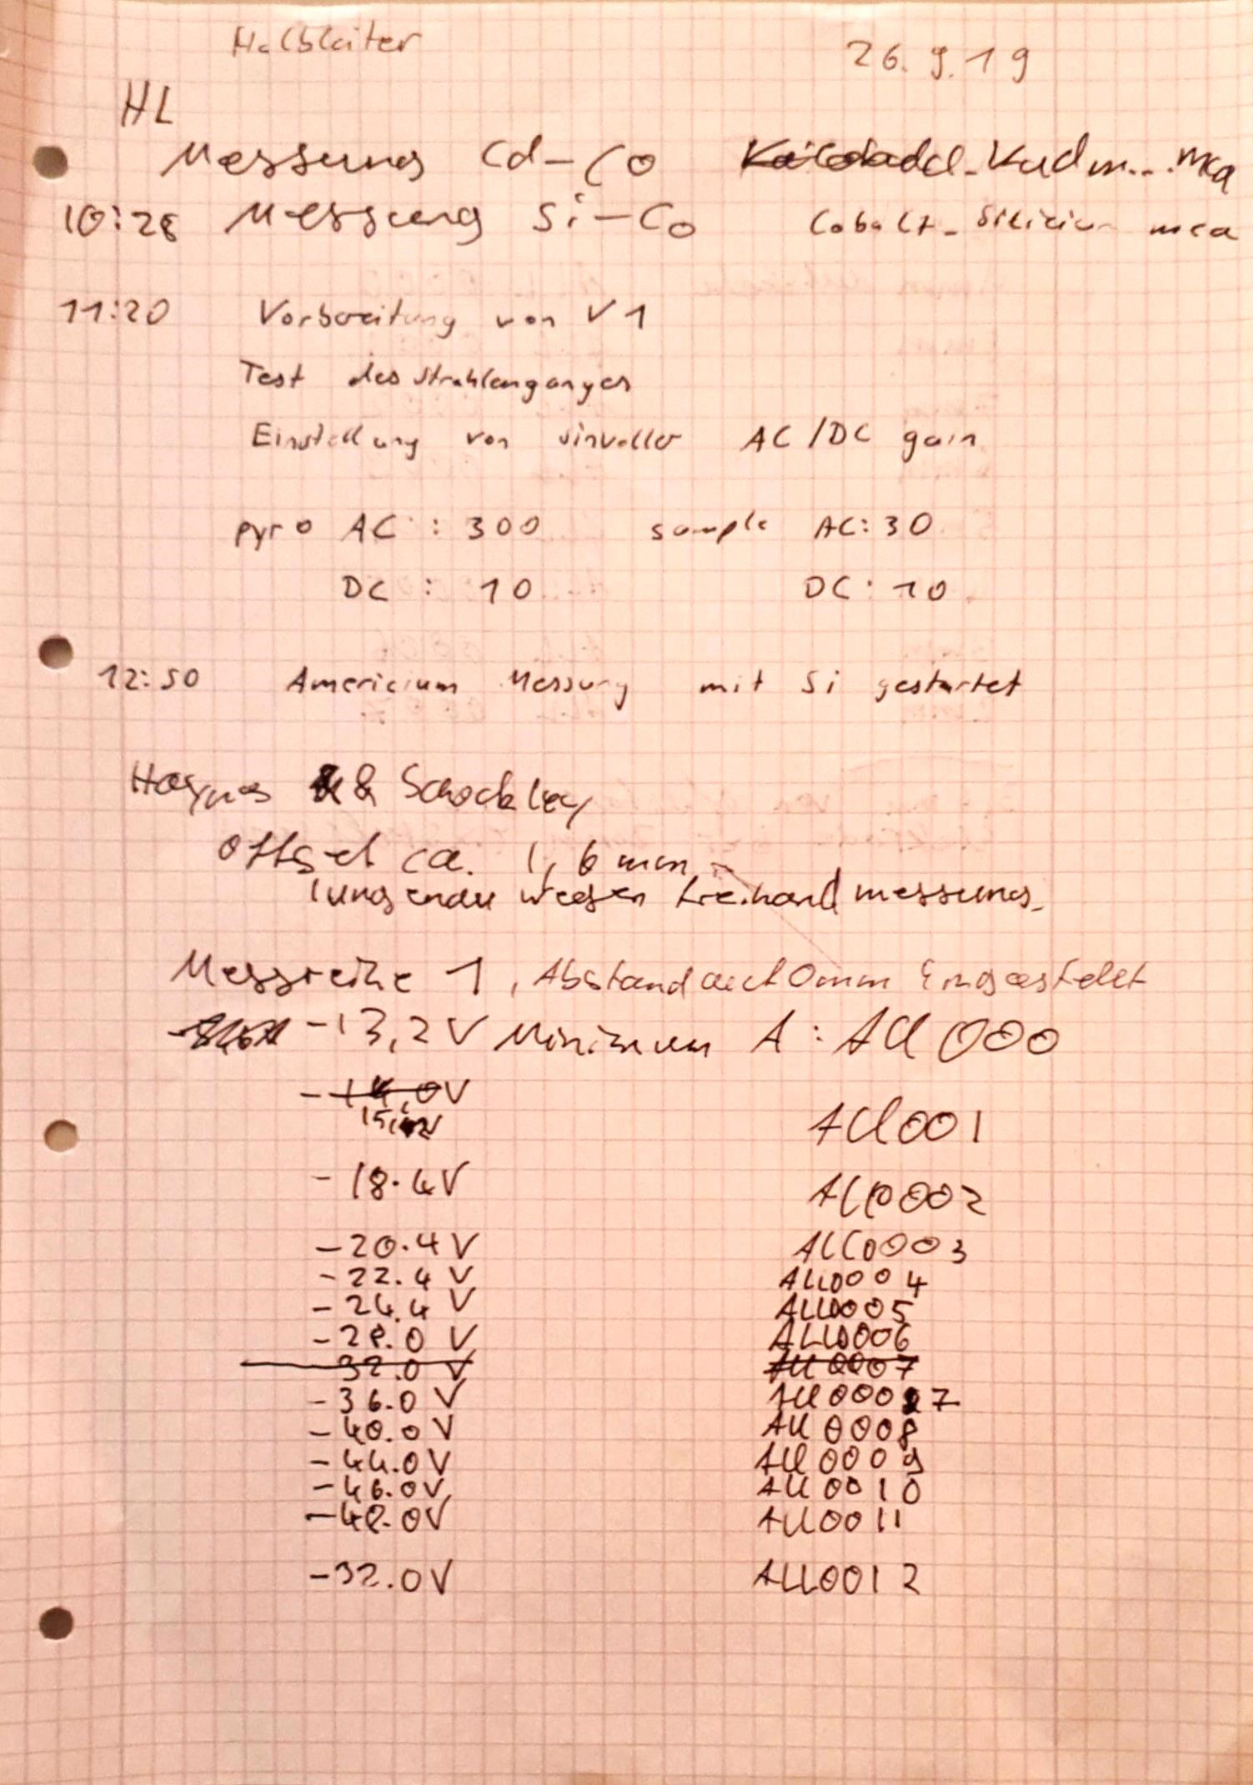
\includepdf[pages=-,scale=0.8]{Bilder/anhang/Halbleiter.pdf}
\end{document}